In this section, we consider the problem which we refer to as \sigla{MCE}{Maximum Covering by Ellipses}. We introduce an algorithm for it, which in fact, works not only for ellipses, but for any disk in a strictly convex normed plane.

\section{Definition}

Axis-parallel ellipses are defined as the set of points that satisfy \autoref{equation:pellipse}. All it takes to describe one is a pair of positive real numbers $(a,b) \in \R_{>0}^2$, with $a>b$, also called its shape parameters, and a center $q \in \R^2$.

An instance of MCE is given by a set of $n$ demand points $\Pp = \{p_1, \dots, p_n\}$, with $p_j\in\R^2$; 
a set of weights $\Ww:=\{w_1, \dots, w_n\}$, with $w_j\in\R_{\ge0}$ being the weight of point $p_j$;
and a set of $m$ axis-parallel ellipses given by their shape parameters $\Rr:=\{(a_1, b_1), \dots, (a_m, b_m)\}$, with $(a_j, b_j)\in\R_{>0}^2$ and $a_j>b_j$.
Additionally, to make the text more clear, we define a set $\E = \{E_1, \dots, E_m\}$, with $E_j : \R^2 \mapsto \R^2$ being a function that takes the center where the $j$-th ellipse is located as input, and returns its coverage region as defined by \autoref{equation:cover_pellipse}.

A solution for MCE is given by $Q:=(q_1, \dots, q_m)\in\R^{2m}$, with $q_j$ being the center of $j$-th ellipse. Let $w : 2^\Pp \mapsto \R_{\ge0}$ as defined by \autoref{eq:subset_w}, then an optimal solution of MCE is given by the optimization problem

\begin{equation*}
	\max_q w\left(\bigcup_{j=1}^m \Pp \cap E_j(q_j)\right).
\end{equation*}

From now on, since ellipses are just unit circles in a strictly convex normed space $(\R^2, ||.||_Q)$, with $||.||_{a, b}$ being an elliptical norm whose unit disk is an ellipse with shape parameters $(a, b)$, we will develop this work for any set of strictly convex unit disks. The following notation is adopted: $D(x)$ represents a unit disk centered at $x\in \R^2$, which is the set of points $\{y \in \R^2 \colon ||y-x|| \le 1 \}$, for any strictly convex plane $(\R^2, ||.||)$, and we denote by $\partial D(x)$, the circle correspondent to that disk.

\section{Related work}
The maximal planar covering using axis-parallel ellipses was first introduced in \citeonline{canbolat} which proposed a mixed integer non-linear programming method for the problem. This first approach showed to be not that efficient as it could not find an optimal solution for some instances within a timeout defined by them. To obtain solutions, not necessarily optimal ones, for the instances which the exact method showed inefficiency, a heuristic technique called Simulated Annealing was used to develop another method. Comparisons were made, which showed that the second approach was able to obtain good solutions, compared to the optimal ones found for some of the instances, within a good run-time.

The second work found in the literature was \citeonline{andreta}, which developed a method that breaks the problem into smaller ones fixing the set of points an ellipse is going to cover. For each set of points fixed as the points an ellipse is going to cover, a small optimization problem is solved to find out if there is a location where the ellipse can be placed, so to cover the set of fixed points. To enumerate the possible solutions and then find an optimal one, the method defined a data structure that stores every set of points an ellipse can cover. This method showed better results and was able to find optimal solutions for the instances that the first method could not get as well as for new created instances.

\section{Maximum Weight Clique}

We introduce in this section a problem equivalent to MCE with only one facility. We refer to this equivalent problem as \sigla{MWC}{Maximum Weight Clique}. This equivalence is also used in the works for MCD in \citeonline{chazelle:1986} and \citeonline{cabello:2006}.

An instance of the \sigla{MWC}{Maximum Weight Clique} is given by a list of points \mbox{$\Pp:=\{p_1,\dots,p_n\}$}, with $p_i \in \R^2$; 
a set of unit disks $\D:=\{D_1(p_1), \dots, D_n(p_n)\}$, with $D_i(p_i)$ being a unit disk in any strictly convex plane; and a set of weights \mbox{$\Ww:=\{w_1, \dots, w_n\}$}, with $w_i\in \R_{>0}$ being the weight of the $i$-th unit disk. We omit the center of a unit disk whenever we are referring to an instance of MWC, that is, $D_i:=D_i(p_i)$.

A clique, in this context, is a non-empty intersection region of one or more disks, and its weight is the sum of the weights of those disks in the intersection.
Following this, a solution for MWC can be defined as just a point $q\in\cup_{j=1}^n D_j$, which is inside any of the given disks in $\D$.
From a solution $q$, the corresponding clique $S$ can be obtained by intersecting every disk that contains $q$ as follows
\begin{equation*}
	S = \bigcap_{j : q \in D_j} D_j.
\end{equation*}
Therefore, an optimal solution of MWC is defined by	$\max_{q} \sum_{D_k \cap q \neq \emptyset} w_k$. 

Let $(\Pp, \Ww, \{(a, b)\})$ be an instance of MCE with only one facility, and $(\Pp, \D, \Ww)$ an instance of MWC, with $\D$ being a set of unit disks in the strictly convex normed space $(\R^2, ||.||_{a,b})$.
If $q_1$ be a solution for the MCE's instance. Then, the disks with centers in $\Pp \cap E_1(q_1)$ have non-empty intersection.
Also, suppose that $q$ is a solution of MWC. Then, the ellipse with shape parameters $(a, b)$ centered at $q$ covers the points, which are the centers of disks, such that $q \in D_j$.
Therefore, both problems are equivalent.

Let us consider the intersection set of $k$ unit disks $\cap_{j=1}^k D_j(x_j)$, for any strictly convex normed space, with $x_j \in \R^2$ being all distinct.
Then, in \citeonline{bi}, two results are stated about that set: its boundary is formed by arcs of unit circles whose centers are in $\{x_1, \dots, x_k\}$, its vertices are in the set $\partial D_i(x_i) \cap \partial D_j(x_j)$, for any $i \neq j$; and $|\partial D_i(x_i) \cap \partial D_j(x_j)| \le 2$, for any $i\neq j$. 
Based on that, we introduce the next definition.

\begin{definicao}
	Let $D_i(p_i)$ and $D_j(p_j)$ be two unit disk in a strictly convex normed space, and $\{\alpha_{ij}^+, \alpha_{ij}^-\} \subset \partial D_i(p_i) \cap \partial D_j(p_j)$,
	 we denote by $\widehat{\alpha_{ij}^+, \alpha_{ij}^-}$ the minimal counter-clockwise arc of $D_i(p_i)$ starting in $\alpha_{ij}^+$ and ending in $\alpha_{ij}^-$. We also refer to $\alpha_{ij}^+$ as an opening intersection point, and to $\alpha_{ij}^-$ as a closing intersection point.
\end{definicao}
Let $\widehat{\alpha_{ij}^+, \alpha_{ij}^-}$ and $\widehat{\alpha_{ij}^-, \alpha_{ij}^+}$ be the two arcs of $\partial D_i$ with respect to the endpoints $\alpha_{ij}^-, \alpha_{ij}^+$.
From \citeonline[Lemma 2]{bi}, we can state that, $\widehat{\alpha_{ij}^+, \alpha_{ij}^-}\subset D_j$, and\\ $\widehat{\alpha_{ij}^-, \alpha_{ij}^+} \cap D_j = \{\alpha_{ij}^-, \alpha_{ij}^+\}$. That is, only the minimal arc is contained in the interior of $D_j$.


Based on that, we are going to develop an algorithm that finds the best clique that $\partial D_i$ is part of, for each $i=1, \dots, n$. Let \mbox{$q_i \in \partial D_i$} be an optimal solution of $\max_{q_i} \sum_{D_k \cap q_i} w_k$. Then, an optimal solution of MWC is just
$\max_{i=1}^n \max_{q_i} \sum_{D_k \cap q_i} w_k$. Notice that this is enough by the results in \citeonline{bi}.

\begin{lema}
	Let $(\Pp, \D, \Ww)$ be an instance of MWC. For each $i\in \{1, \dots, n\}$,
	if there is \mbox{$j \in \{1, \dots, n\}$}, $j\neq i$, such that $D_i \cap D_j \neq \emptyset$, then, for any solution $q_i \in \partial D_i$, let $J=\{j \colon q_i \in D_j\}$,
	$q_i \in \cap_{j \in J, j\neq i}\{\widehat{\alpha_{ij}^+, \alpha_{ij}^-}\}$.
\end{lema}

\begin{proof}
	Suppose that $q_i \not \in \widehat{\alpha_{ij}^+, \alpha_{ij}^-}$, for some $j \in J\setminus \{i\}$.
	By definition $q_i \in \partial D_i$, and by \citeonline[Lemma 2]{bi}, we have that $q_i \in \widehat{\alpha_{ij}^-, \alpha_{ij}^+}$, which implies that $q_i \in \{\alpha_{ij}^-, \alpha_{ij}^+\}$, which would imply that  $q_i \in \widehat{\alpha_{ij}^+, \alpha_{ij}^-}$, contradicting the assumption we made.
\end{proof}


For the algorithm, for each $i$, instead of looking for $q_i$, we are going to construct the best subset $J \in \{1, \dots, n\}$. This idea is based on the algorithms proposed in \citeonline{drezner} and \citeonline{cabello:2006}. Let us consider the following circular list
\begin{equation*}
	A_i = \{\alpha_{ij}^+ \colon j\neq i, D_i \cap D_j \neq \emptyset\} \cup \{\alpha_{ij}^- \colon j\neq i, D_i \cap D_j \neq \emptyset \}.
\end{equation*}
Suppose that $A_i$ is sorted by the angles of $D_i$ in $[0, 2\pi)$ corresponding to each intersection point, breaking ties by prioritizing opening ones.
Finding the best solution which $D_i$ is part of can be done by traversing $A_i$ while keeping a set of active disks. When an opening intersection angle is reached, the corresponding disk is added to the active set; and when a closing one is seen, the corresponding disk is removed from the active set. This way, finding an optimal solution can be achieved by keeping the weight of the active disks as well as the best clique found so far.

In practice, traversing a circular list can be emulated by traversing a regular list that has a copy of the original circular list added to its end. 
Therefore, the list $B_i$ is defined here as a list that contains the elements of $A_i$ and a copy of it shifted to the interval $[2\pi, 4\pi]$. It is defined as
\begin{equation}\label{eq:bi2}
B_i = A_i\cup\bigcup_{j\neq i} \{2\pi+\alpha_{ij}^+ \colon j\neq i, D_i \cap D_j \neq \emptyset\} \cup \{2\pi+\alpha_{ij}^- \colon j\neq i, D_i \cap D_j \neq \emptyset \}.
\end{equation}
Assuming $B_i$ is sorted with the same criteria as $A_i$, a simple traversal, starting at the first element and going until the last one, simulates a traversal on the circular list $A_i$.
This works because for any pair of disks $D_i$, $D_j$; $B_i$ contains $\alpha_{ij}^+ < \alpha_{ij}^- + 2\pi$. That is, the algorithm encounters an opening intersection point before reaching a closing one for any circle.

In \autoref{fig:array_disks2}, the intersection points between $\partial D_1$ (solid border) with $\partial D_2, \partial D_3$, and $\partial D_4$ (dashed border) are shown with a plus or minus sign indicating opening or closing intersection points. 
The intersection list $B_1$ is also displayed in \autoref{fig:array_disks2} along with the size of the set of active disks $Q$ after processing a point in $B_1$.
It is possible to see that the optimal clique highlighted in \autoref{fig:array_disks2} is enclosed by the arcs defined by $\alpha_{14}^+$ and $\alpha_{14}^-$, and can also be identified by following $B_1$ while keeping track of $Q$.
The special intersection point of $\partial D_1$ with itself can also be seen in \autoref{fig:array_disks2}. Its usage is very convenient as with $\alpha_{11}^+$ and $\alpha_{11}^-$  in $B_1$, the algorithm inserts $D_1$ in the set of active disks before processing any point, and removes $D_1$ only after every point has been processed.

\begin{figure}[!htb]
	\centering
	
	\caption{The intersection list of a disk with three other disks.}
	%\usetikzlibrary{matrix}



\tikzset{every picture/.style={line width=0.75pt}} %set default line width to 0.75pt        

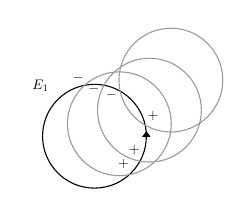
\begin{tikzpicture}[x=0.75pt,y=0.75pt,yscale=-1,xscale=1]
%uncomment if require: \path (0,95); %set diagram left start at 0, and has height of 95

%Shape: Circle [id:dp37777408295388804] 
\draw   (21,59.5) .. controls (21,45.69) and (32.19,34.5) .. (46,34.5) .. controls (59.81,34.5) and (71,45.69) .. (71,59.5) .. controls (71,73.31) and (59.81,84.5) .. (46,84.5) .. controls (32.19,84.5) and (21,73.31) .. (21,59.5) -- cycle ;
%Shape: Circle [id:dp4562198988843913] 
\draw  [color={rgb, 255:red, 155; green, 155; blue, 155 }  ,draw opacity=1 ] (47.5,46.94) .. controls (47.5,33.14) and (58.69,21.94) .. (72.5,21.94) .. controls (86.31,21.94) and (97.5,33.14) .. (97.5,46.94) .. controls (97.5,60.75) and (86.31,71.94) .. (72.5,71.94) .. controls (58.69,71.94) and (47.5,60.75) .. (47.5,46.94) -- cycle ;
%Shape: Circle [id:dp8913971633985722] 
\draw  [color={rgb, 255:red, 155; green, 155; blue, 155 }  ,draw opacity=1 ] (33,53.5) .. controls (33,39.69) and (44.19,28.5) .. (58,28.5) .. controls (71.81,28.5) and (83,39.69) .. (83,53.5) .. controls (83,67.31) and (71.81,78.5) .. (58,78.5) .. controls (44.19,78.5) and (33,67.31) .. (33,53.5) -- cycle ;
%Shape: Circle [id:dp05970043129919356] 
\draw  [color={rgb, 255:red, 155; green, 155; blue, 155 }  ,draw opacity=1 ] (57.81,32.47) .. controls (57.81,18.66) and (69,7.47) .. (82.81,7.47) .. controls (96.62,7.47) and (107.81,18.66) .. (107.81,32.47) .. controls (107.81,46.27) and (96.62,57.47) .. (82.81,57.47) .. controls (69,57.47) and (57.81,46.27) .. (57.81,32.47) -- cycle ;
%Straight Lines [id:da04725899028195979] 
%\draw[densely dotted]  (21,59.5) -- (71,59.5) ;


%Flowchart: Extract [id:dp5267407418119328] 
\draw  [fill={rgb, 255:red, 0; green, 0; blue, 0 }  ,fill opacity=1 ] (71,57.45) -- (72.52,59.55) -- (69.48,59.55) -- cycle ;

\draw (60,73) node [scale=0.5]  {$+$};
% Text Node
\draw (65.22,66) node [scale=0.5]  {$+$};
% Text Node
\draw (74.22,50) node [scale=0.5]  {$+$};
% Text Node
\draw (54.22,39.56) node [scale=0.5]  {$-$};
% Text Node
\draw (45.62,36.96) node [scale=0.5]  {$-$};
% Text Node
\draw (38.02,31.56) node [scale=0.5]  {$-$};


% Text Node
\draw (20,35) node [scale=0.5]  {$E_{1}$};
\end{tikzpicture}

\begin{tikzpicture}

\matrix [matrix of nodes,row sep=,row sep=0mm,
column 1/.style={nodes={rectangle,draw,minimum width=1.5em, minimum height=0.5em}},
column 2/.style={nodes={rectangle,draw,minimum width=1.5em, minimum height=0.5em}},
column 3/.style={nodes={rectangle,draw,minimum width=1.5em, minimum height=0.5em}},
column 4/.style={nodes={rectangle,draw,minimum width=1.5em, minimum height=0.5em}},
column 5/.style={nodes={rectangle,draw,minimum width=1.5em, minimum height=0.5em}},
column 6/.style={nodes={rectangle,draw,minimum width=1.5em, minimum height=0.5em}},
column 7/.style={nodes={rectangle,draw,minimum width=1.5em, color=gray, minimum height=0.5em}},
column 8/.style={nodes={rectangle,draw,minimum width=1.5em, color=gray, minimum height=0.5em}},
column 9/.style={nodes={rectangle,draw,minimum width=1.5em, color=gray, minimum height=0.5em}},
column 10/.style={nodes={rectangle,draw,minimum width=1.5em, color=gray, minimum height=0.5em}},
column 11/.style={nodes={rectangle,draw,minimum width=1.5em, color=gray, minimum height=0.5em}},
column 12/.style={nodes={rectangle,draw,minimum width=1.5em, color=gray, minimum height=0.5em}}
] (O)
{
$+$ & $-$ & $-$ & $-$ & $+$ & $+$ & $+$ & $-$ & $-$ & $-$ & $+$ & $+$\\
%$+$ & $-$ & $-$ & $-$ & $+$ & $+$\\
};

\node at (-4,-0.5) {$0$};
\node at (0,-0.5) {$2\pi$};
\end{tikzpicture}
	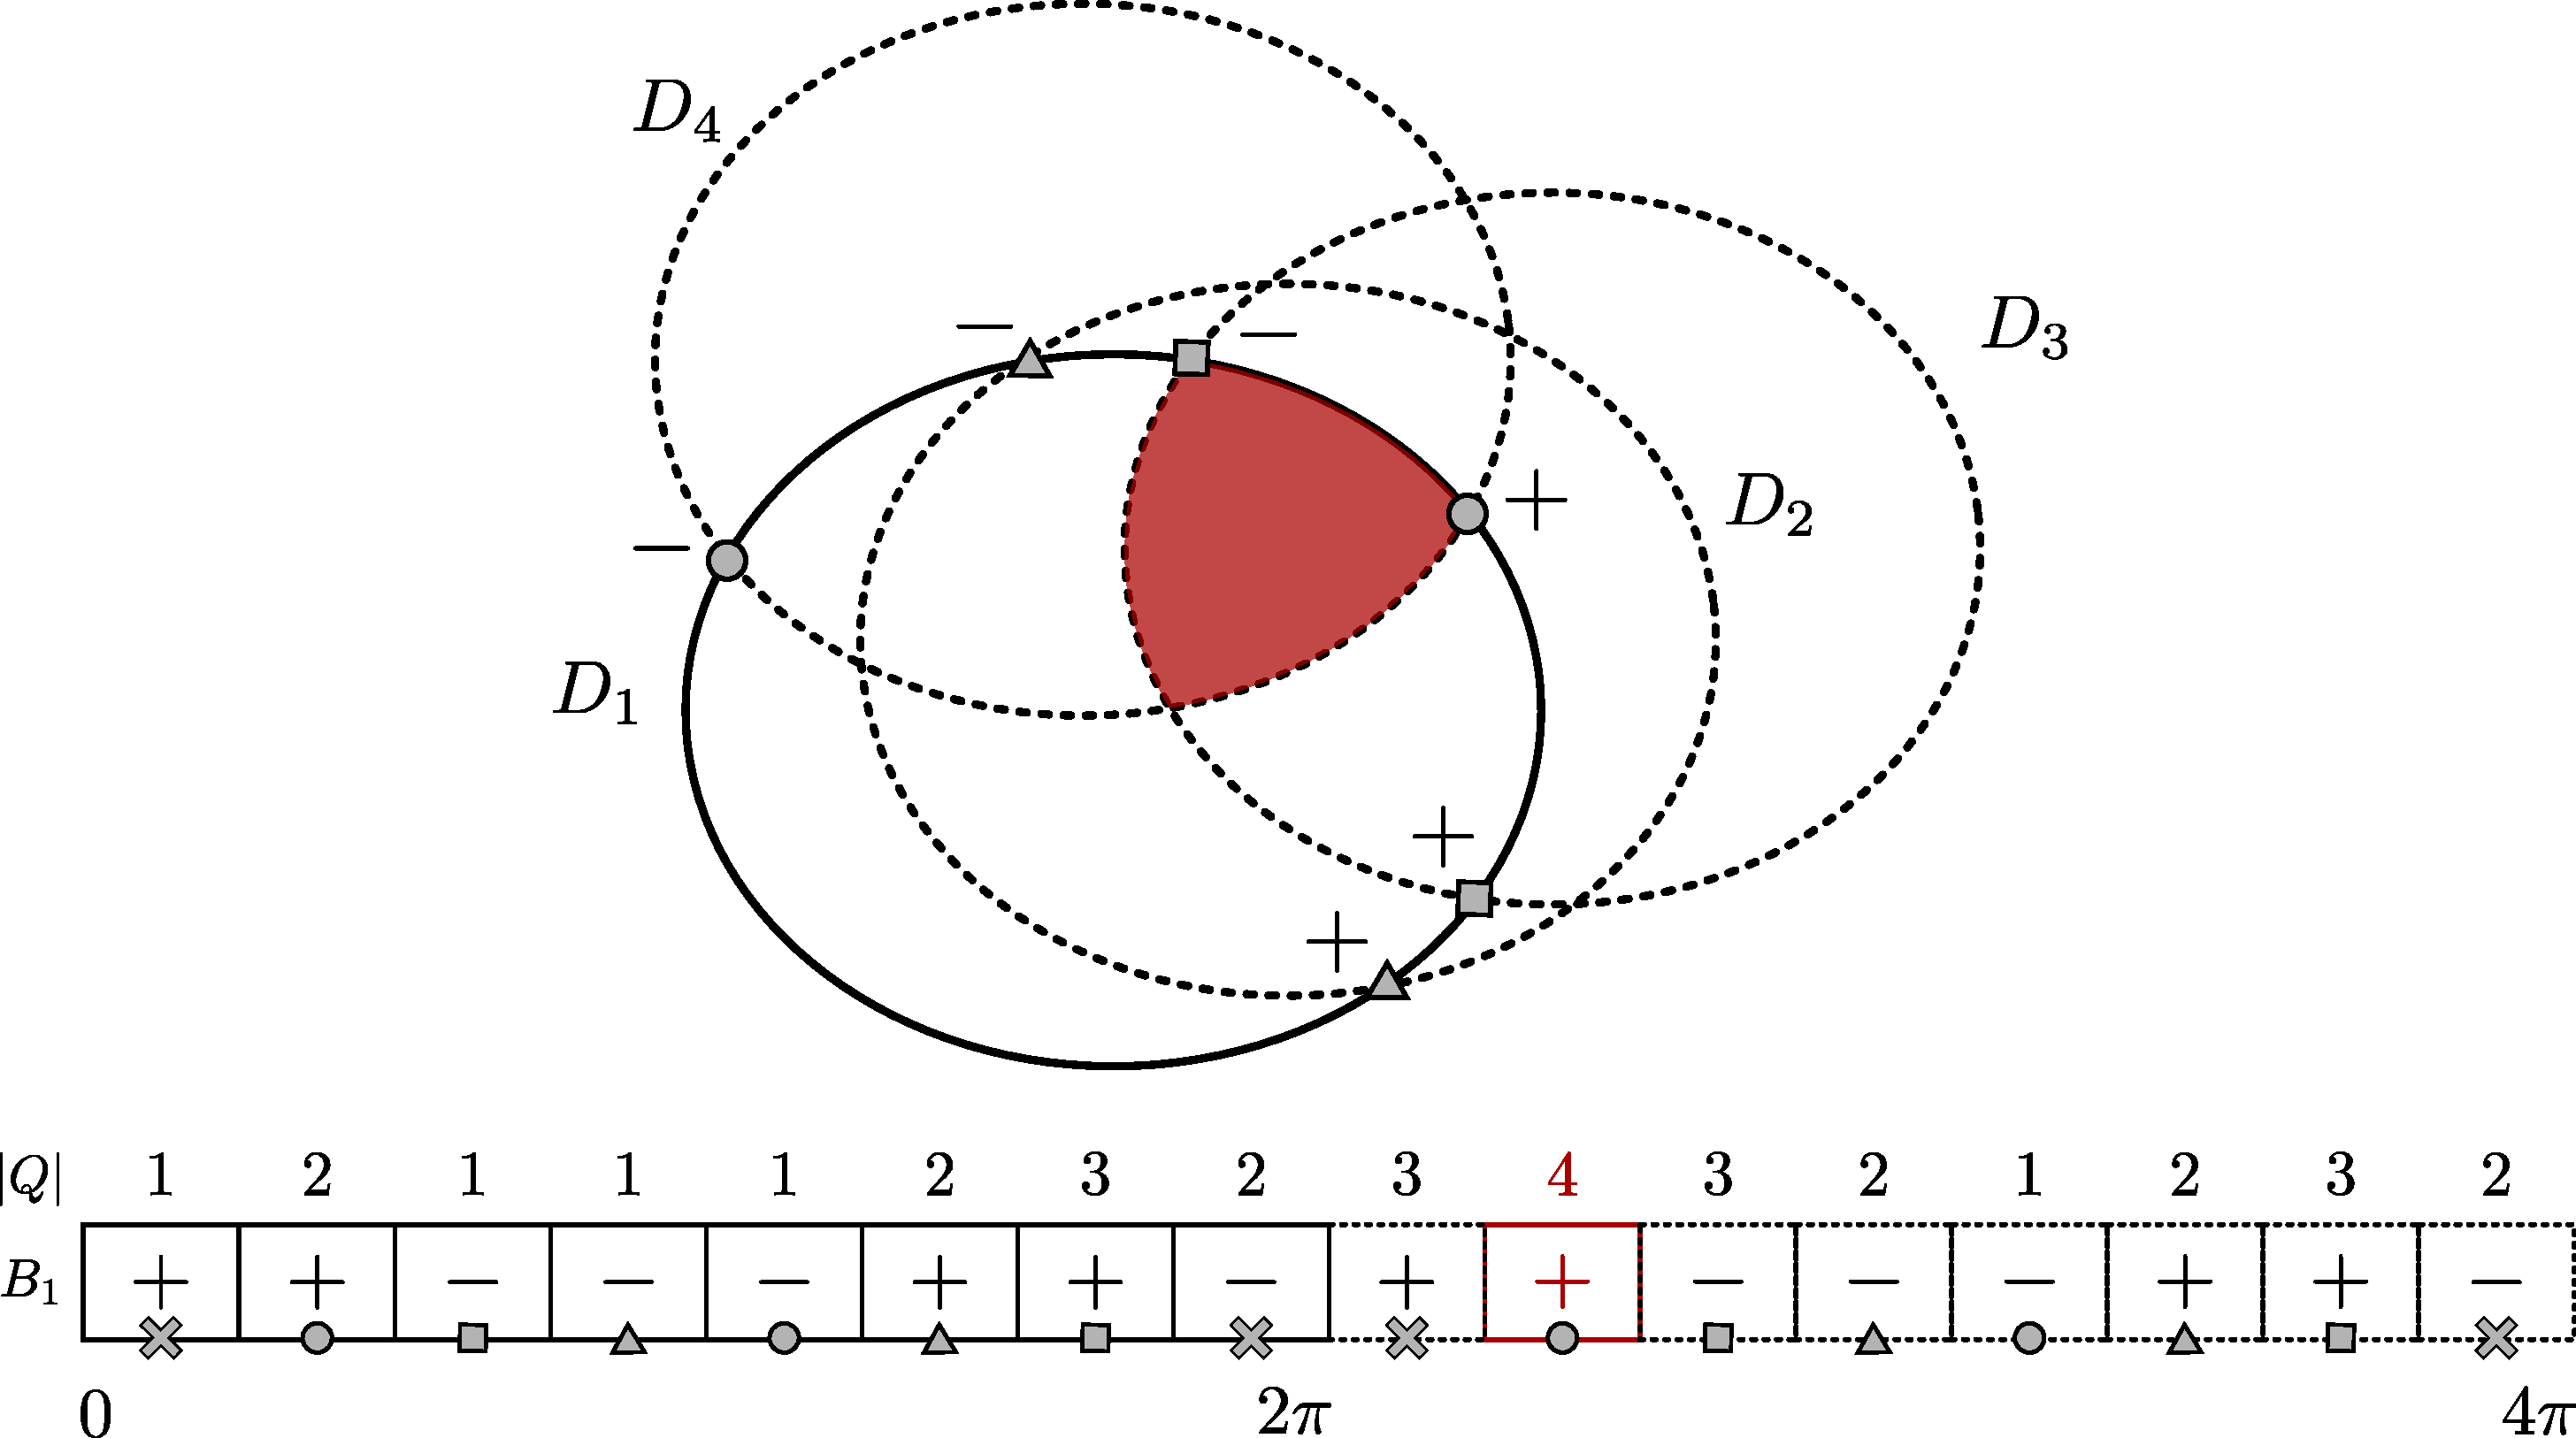
\includegraphics[scale=.3]{tex/figures/3_disks_intersect_.pdf}
	\fautor
	\label{fig:array_disks2}
\end{figure}

%\begin{algoritmo}[!htb]
%	\caption{Algorithm for MWC.}\label{algoritmo:mwc}
%	\begin{algorithmic}[1]
%		\Require{A set of points $\Pp=\{p_1,\dots,p_n\}$, and a set of weights $\Ww=\{w_1, \dots, w_n\}$.}
%		\Ensure{A point that is inside the maximum weight clique of unit disks.}
		
%		\item[]
		
%		\Procedure{$MWC$}{$\Pp, \Ww$}
%		\State Let $\D=\{D_1, \dots, D_n\}$ be a set of unit disks, with centers in $\Pp$ and weights in $\Ww$
		
%		\State $Q_{best} \gets \{\}$
%		\State $q^* \gets$ $p_1$
%		\ForAll{$D_i \in \D$}
%		\State Let $B_i$ be the list of intersection angles of $D_i$ as defined by \autoref{eq:b_i}
		
%		\State $Q \gets \{\}$ \Comment{The set of active disks.}
%		\For{$\alpha \in B_i$}\Comment{Assuming $B_i$ is sorted.}
%		\State Let $D_j$ be the disk, such that $\theta \in D_j\cap D_i$
%		\If{$\theta$ is a opening angle}
%		\State $Q \gets Q \cup \{D_j\}$
%		\Else
%		\State $Q \gets Q \setminus \{D_j\}$
%		\EndIf
%		\If{$w(Q_{best}) < w(Q)$} 
%		\State $Q_{best} \gets Q$
%		\State $q^* \gets$ point corresponding to the intersection angle $\theta$
%		\EndIf
%		
%		\EndFor
%		\EndFor
		
%		\State \Return $q^*$
%		\EndProcedure
%	\end{algorithmic}
%\end{algoritmo}

\section{From MWC to MCE}

Now we are going to modify the algorithm for MWC to work as a basis for the algorithm for multiple disks.
Suppose that an instance $(\Pp, \Ww, \Rr)$ of MCE is given. For each ellipse with shape parameters $(a_j, b_j)$, we have the instance $(\Pp, \D, \Ww)$ of MWC, with $\D$ being a set of unit disks from a strictly convex normed space where the unit disk is an axis-parallel ellipse with shape parameters $(a_j, b_j)$.

\begin{definicao}
	Let $(\Pp, \Ww, \Rr)$ be an instance of MCE. For each $j \in \{1, \dots, m\}$, let $(\Pp, \D, \Ww)$ be the equivalent instance of MWC using the $j$-th ellipse as their unit disk, we define as the \sigla{CLS}{Candidate List Set} $S_j$ for $j$-th ellipse as
	\begin{equation*}
	S_j = \bigcup_{i=1}^n \{\alpha_{ik}^+ \colon k\neq i, D_i \cap D_k \neq \emptyset\}\cup \{p_i\}.
	\end{equation*}
\end{definicao}

Based on this, we introduce a theorem that allows us to develop an algorithm for MCE based on the developments we made for MWC.

\begin{theorem}\label{th:mce2}
	Let $(\Pp, \Ww, \Rr)$ be an instance of MCE, and $\Omega(\Pp, \Ww, \Rr)$ be a set of solutions defined as 
	\begin{equation*}\label{eq:omega2}
		\Omega(\Pp, \Ww, \Rr) = \{Q\in \R^{2m} \colon q_j \in S_j \textnormal{ for all } j\in\{1, \dots, m\}\},
	\end{equation*}
	Then there exists an optimal solution $Q^*\in \Omega(\Pp, \Ww, \Rr)$, and $|\Omega(\Pp, \Ww, \Rr)|\le n^{2m}$.
\end{theorem}
\begin{proof}
		Notice that $\Omega(\Pp, \Ww, \Rr)$ is defined as the combination of every possible solution from each CLS. To prove that it contains an optimal solution $Q^*$, it is enough to prove that for all $j\in\{1, \dots, m\}$, there exists $q_j\in S_j$, such that $\Pp \cap E_j(q_j^*) \subset \Pp \cap E_j(q_j)$. That is, we only need to show that the CLS of every ellipse contains a center that makes the ellipse cover the same points (possibly some additional ones) that it covers in an optimal solution.
		We ignore the case where an ellipse does not cover any points.
		
		First case: $|\Pp \cap E_j(q_j^*)|=1$. This case is included in $S_j$ as it contains the possible solutions where the center of the ellipse is the actual points in $\Pp$.
		
		Second case: $|\Pp \cap E_j(q_j^*)| > 1$. Let $X = \{i \colon p_i \in \Pp \cap E_j(q_j^*)$. In the equivalent instance of MWC, we have that $\cap_{i\in X} D_i \neq \emptyset$ is a region bounded by arcs of circles with centers in $\Pp \cap E_j(q_j^*)$ with vertices being pairwise intersections of $\partial \D$, with at least one of them being an opening intersection point.
		
		Lastly, we have that $|S_j| \le \binom{n}{2} + n = \frac{n(n+1)}{2} \le n^2$. Therefore,
		$|\Omega(\Pp, \Ww, \Rr)| \le |S_1|\times \dots \times |S_m| \le n^{2m}$.
\end{proof}

\section{An algorithm for MCE}

First, we describe, based on \autoref{th:mce2}, an algorithm to return the CLS for every ellipse. This algorithm runs in $\bigO(n)$, and is based on the idea used on the development of the algorithm for MWC.

\begin{algoritmo}
	\caption{Algorithm that returns a CLS for a disk.}\label{algoritmo:mce_cls}
	\begin{algorithmic}[1]
		\Require{A set of points $\Pp=\{p_1,\dots,p_n\}$ with weights $\Ww=\{w_1, \dots, w_n\}$, and the shape parameters $(a, b)\in\R_{>0}^2$.}
		\Ensure{A CLS for the axis-parallel ellipse.}
		
		\item[]
		
		\Procedure{CLS-MCE}{$\Pp, \Ww, (a,b)$}
		\State Let $\D$ be a set of unit disks on the strictly convex normed space $(\R^2, ||.||_{a,b})$.
		\State $S \gets \{\}$
		\ForAll{$p_i \in \Pp$}
		\State $S \gets S \cup \{p_i\}$
		
		\ForAll{$j \neq i \colon D_j \cap D_i \neq \emptyset$}

		\State $S \gets S \cup \{\alpha_{ij}^+\}$	

		\EndFor
		\EndFor
		
		\State \Return $S$
		\EndProcedure
	\end{algorithmic}
\end{algoritmo}

Then, we define in \autoref{algoritmo:mce2}, an algorithm for MCE, which backtracks to find an optimal solution taking into account every possibility in the CLS of every ellipse. This way, we obtain a $\bigO(mn^{2m+1})$ algorithm for MCE.

\section{Determining $\alpha_{ij}^+$ and $\alpha_{ij}^-$}\label{section:ellipses_intersection2}

Let $E_1(q_1)$, and $E_2(q_2)$ be two coverage region of ellipses centered at $q_1, q_2\in\R^2$ respectively, with shape parameters $(a, b)\in\R^2_{>0}$. After changing the coordinates to make the center of the first ellipse be at the origin, the intersection points between the two ellipses are defined by

\begin{align}
	\frac{x^2}{a^2} + \frac{y^2}{b^2} = 1 && (E_1) \label{eq:ell_inter_1}\\
	\frac{(x-h)^2}{a^2} + \frac{(y-k)^2}{b^2} = 1 && (E_2), \nonumber
\end{align}
where $(h,k)\in\R^2$ is the center of the second ellipse after the coordinates were translated by $-q_1$. As both equations are equal to $1$, we have
\begin{align}
	b^2x^2 + a^2y^2 &= b^2(x-h)^2 + a^2(y-k)^2 \nonumber\\
	x &= y\frac{-2ka^2}{2hb^2} + \frac{b^2h^2 + a^2k^2}{2hb^2} \nonumber\\
	x &= y\alpha + \beta.\label{eq:ell_inter_2}
\end{align}
Replacing \autoref{eq:ell_inter_2} into \autoref{eq:ell_inter_1}, we get
\begin{align}\label{eq:ell_inter_3}
	y^2(b^2\alpha^2 + a^2) + y(2\beta\alpha b^2) + b^2\beta^2 -a^2b^2 = 0,
\end{align}
which is a second degree polynomial. Then, $\partial E_1(q_1) \cap \partial E_2(q_2) \neq \{\}$ if, and only if the roots of \autoref{eq:ell_inter_3} are real. The intersection points itself can be obtained by solving the polynomial for $y$ and plugging its value back into the $x=y\alpha + \beta$ equation.

Suppose that $\partial E_1(q_1) \cap \partial E_2(q_2) = \{p_1, p_2\}$, with $p_1 \neq p_2$. To determine $\Gamma_+(1,2)$ and $\Gamma_-(1,2)$, we need to first determine the intersection angles corresponding to $p_1$ and $p_2$ on $E_1(q_1)$. 

Let $\gamma_1$ and $\gamma_2$ be two curves defined as \autoref{eq:parametric_ellipse} for $E_1(q_1)$ and $E_2(q_2)$ respectively. 
The intersection angle of $p_i$ in $E_j(q_j)$ is defined as $t_i^{(j)} \in [0, 2\pi)$, such that $\gamma_j(t_i^{(j)}) = p_i$, for $i, j \in \{1, 2\}$. Obtaining $t_i^{(j)}$ can be done analytically solving the equation

\begin{equation}\label{eq:angle_inter}
	\dfrac{a}{b}\dfrac{p_{iy}-q_{jy}}{p_{ix}-q_{jx}} = \tan{(t_i^{(j)})}.
\end{equation}

Determining which one of the points is $\alpha_{ij}^+$, we just need to use the assumption that $\widehat{\alpha_{ij}^+, \alpha_{ij}^-}$ is minimal. This can be done using the angle of the intersection points obtained from \autoref{eq:angle_inter}. 

\begin{algoritmo}
	\caption{Algorithm for MCE}\label{algoritmo:mce2}
	
	\begin{algorithmic}[1]
		\Require{A set of points $\Pp=\{p_1,\dots,p_n\}$, a list of weights $\Ww=\{w_1, \dots, w_n\}$, and a list of shape parameters $\Rr=\{(a_1, b_1), \dots, (a_m, b_m)\}$.}
		
		\Ensure{An optimal solution for MCE.}
		
		\item[]
		\Procedure{$MCE$}{$\Pp, \Ww, \Rr$}
		\State \Return $MCE_{bt}(\Pp, \Ww, \Rr, 1)$
		\EndProcedure
		\State
		\Procedure{$MCE_{bt}$}{$Z, \Ww, \Rr, j$}
		\If{$j = m+1$}
		\State \Return $0$
		\EndIf
		
		\State $(q_j^*, \dots, q_m^*) \gets (0, \dots, 0)$
		
		\State $S_j \gets \textnormal{CLS-MCE}(Z, a_j, b_j)$
		\For{$q_j \in S_j$}
		\State $Cov \gets \Pp \cap E_j(q_j)$
		\State $(q_{j+1}, \dots, q_m) \gets MCE_{bt}(Z \setminus Cov, \Ww, \Rr, j+1)\}$
		
		\If{$w(\cup_{k=j}^m Z \cap E_k(q_k)) >  w(\cup_{k=j}^m Z \cap E_k(q_k^*))$}
		\State $(q_j^*, \dots, q_m^*) \gets(q_j, \dots, q_m)$
		\EndIf
		\EndFor
		
		\State \Return $(q_j^*, \dots, q_m^*)$
		\EndProcedure
	\end{algorithmic}
\end{algoritmo}